\section{Durchführung}
\label{sec:Durchführung}

Der Versuch besteht aus einem Kreislauf aus Acryl Rohren und Schläuchen, durch den ein Gemisch aus Wasser, Glycerin und Glaskugeln fließt. Die Flüßigkeit wird von
einer Zentrifugalpumpe angetrieben. Die Fleißgeschwindigkeit ist hierbei einstellbar.

\begin{figure}[H]
	\centering
	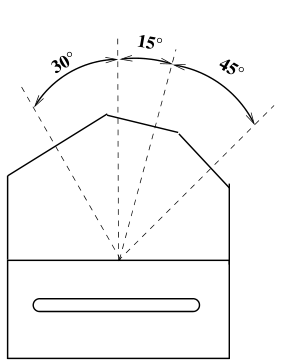
\includegraphics[width=0.6\linewidth]{data/prisma.png}
	\caption{Doppler-Prisma mit Winkeln.}
	\label{fig:prism}
\end{figure}
\noindent
Es wird ein ebenfalls aus Acryl bestehendes Doppler-Prisma, wie in \autoref{fig:prism} verwendet, um die Schallsonde in einem reproduzierbaem Winkel mit dem Rohr zu koppeln.
Alle Abstände der verschiedenen Flächen des Prismas zum Rohr sind hierbei identisch.
\newline
Zum Senden und Empfangen von Ultraschallwellen wird in diesem Versuch eine, an einen Doppler-Generaor angeschlossene und zur Auslesung von Daten mit einen Computer verbundene
$2\si{\mega\Hz}$ Schallsonde verwendet. Die Messdaten werden am Computer mit dem Programm Flowview dargestellt und gespeichert.
\newline
Auf jegliche Flächen zwischen Rohr, Prisma und Schallsonde wird Ultrschallgel aufgetragen, um die Absorbtion von Schall durch die Luft zu minimieren.
\newline\newline
Der ersten Teil des Versuches besteht darauß, die Strömungsgeschwindigkeit der Flüßigkeit durch das Acryl Rohr für fünf verschiedene Leistungsstufen der Zentrifugalpumpe zu
bestimmen. Die Messung für alle fünf Geschwindigkeiten werden jewils an allen dreien in \autoref{fig:prism} zu sehenden Winkeln durchgeführt.
\newline
Es wird hierzu die Schallsonde unter Verwendung von Ultraschallgel an das Doppler-Prisma gekoppelt und am Doppler-Generator ein Sample-Volume von Large eingestellt. Im
Anschluss kann die Zentrifugalpumpe auf bestimmte Leistungswerte eingestellt werden. Diese werden zusammen mit den zugehörigen Messwerte der Schallsonde für die Frequenzen
am Computer gespeichert.
\newline\newline
Im zweiten Teil des Versuches wird nun das Strömungsprofil der Dopplerflüssigkeit bestimmt. Es wird die Schallsonde mit dem Doppler-Prisma gekoppelt und das Sample-Volume
auf Small gestellt. Die Zentrifugalpumpe wird zunächst auf 70\% der Maximalleistung eingestellt, wobei im Anschluss eine identische Messreihe mit 45\% durchgeführt
wird.
\newline
Zur Messung des Strömungsprofils muss die Messtiefe der Schallsonde variirt werden. Sie wird von $12\si{\micro\s}$ auf $20\si{\micro\s}$ in Schritten
von $0,5\si{\micro\s}$ erhöht. Die Messwerte der Streuintensität und Momentangeschwindigkeit werden jeweils mit den zugehörigen Messtiefen vom Computer abgelesen und
notiert.